\section{Attack Description}\label{sec:attack}

To successfully attack these systems, an attacker needs to overshadow the wireless channel to manipulate the raw demodulated data.
Depending on their goals, the attacker can either generate the signal to be injected beforehand or in real time.
Generating the data beforehand does not require a receiver, only hardware capable of transmitting, but does require that the attacker generate their own data or find relevant prior broadcasts to manipulate and replay.
Alternatively, with the addition of their own receiver dish, an attacker can receive the broadcast themselves and process it in real time to add artifacts or mask specific properties of the signal.

% TODO: find that paper somewhere about generating convincing satellite images
The injected data is designed to either poison the derived datasets or to exploit processing stages in the decoding pipeline.
Convincingly poisoning the derived datasets requires that the overshadowed waveform decodes to raw data which is sufficiently similar to the original.
This may prove easier in the real-time setup, in which the attacker can selectively modify only the relevant part of the signal.
Exploiting the processing stages, however, generally relies on creating malformed protocol headers to manipulate control flow in the software.
This must be done beforehand by discovering vulnerabilities in the processing stack and crafting the required packets.

% Call forward to the evaluation section
In the case of FIRMS, the satellite-derived dataset is a map of active forest fires, each with coordinates and a confidence value.
The dataset is derived primarily from the infrared bands of the MODIS sensor, which can reveal hotspots on the surface.
We consider the scenarios of injecting ficticious forest fires and masking existing ones, both in the pre-prepared and real-time setups.
We also perform a security analysis of the decoding software itself, demonstrating how vulnerabilities in the protocol handling can lead to denial of service and arbitrary code execution upon reprocessing.

\subsection{Affecting satellite-derived datasets}

To affect a derived dataset such as forest fire detection, the attacker needs to inject a signal that decodes to the desired raw data.
This data must target the algorithm responsible for generating the desired dataset, causing it to misclassify its input.
This leads to effects such as the detection of ficticious forest fires, and the masking of existing ones. %TODO: rephrase? masking isn't really the opposite of detection

Where the raw data is used for generating multiple derived datasets, the attacker may need to be careful to ensure that the injected data sufficiently resembles legitimate data to avoid detection. % TODO: rewrite - data, data, data...
For example, the MODIS data is used to generate color-corrected images of the Earth's surface, with the forest fire data rendered on top.
If the images appear out of sequence, distorted, or not like the Earth's surface at all, the downstream services which rely upon the data are unlikely to trust it.

As a result, we assume that for this case the attacker begins with instrument data that is sufficiently close to the original signal.
The means for obtaining such data include replaying old data, generating new convincing data, or running the attack setup in real time.
% These different approaches, and their advantages and drawbacks, are discussed in Section~\ref{sec:evaluation}.

% Getting the images to not appear distorted can itself be a challenge
% We can show the scan line problem for this

% TODO: some diagram of the packet and its fields?

Once this data has been obtained, the attacker needs to determine how to manipulate the instrument data, and then reencode it according to the packet protocol.
Each satellite system and instrument is likely to use its own custom protocol for its data channel.
In the case of MODIS, the format consists of an extension to the CCSDS \textit{Space Packet Protocol} (SPP), the dominant network layer protocol for space and satellite systems~\cite{modisDescription},p177.

After the primary header, a secondary header is used to encode timing information alongside information about the packet type and location in the overall image.
The sensor readings are represented as a densely packed array of 12-bit words within the data zone, with a trailing checksum.
Each value represents the intensity of light incident to the sensor of a specific frequency band, which is indicated by the position of the word within the array~\cite{modisDescription},p183-189.

FIRMS derives its dataset from the \textit{MODIS Active Fire Product Science Processing Algorithm} (MOD14\_SPA), which primarily uses the bands of 4 and 11 micrometer wavelengths in the infrared spectrum to detect hotspots.
Therefore, in order to manipulate the detected fires whilst leaving the visible images untouched, the attacker only needs to affect the values in these channels and recalculate the checksum.
%other bands are used are used for the rejection of false positives, and could theoretically be manipulated for finer-grained control.

Once the falsified data has been created, the attacker needs to reencode it according to the packet protocol used.
For Terra and Aqua, the MODIS data is already in the network layer protocol SPP, which must then be acked into data link layer frames for broadcast.
Satellites such as those in the EOS fleet implement a custom data link layer protocol, fine-tuned to their operational requirements.

\begin{figure*}
    \centering
    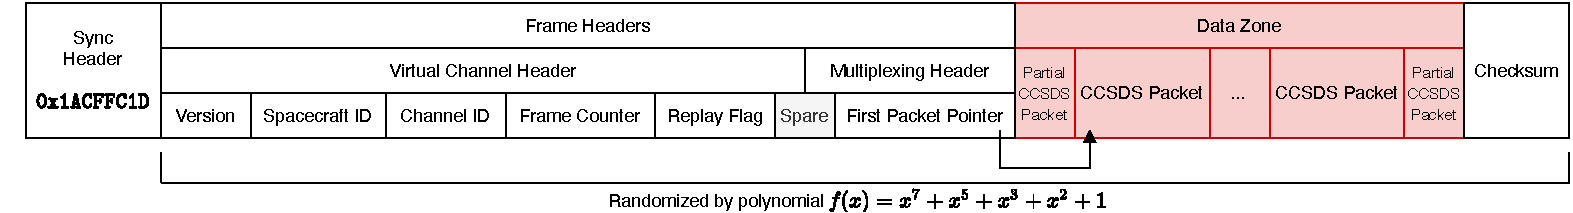
\includegraphics[width=\textwidth]{diagrams/cadu_diagram.pdf}
    \caption{Layout of data within a Channel Access Data Unit (CADU). The section marked in red can contain arbitrary attacker-specified data.}
    \label{fig:cadu_diagram}
\end{figure*}

Terra and Aqua make use of the custom \textit{Channel Access Data Unit} (CADU) protocol shown in Figure~\ref{fig:cadu_diagram}, a fixed-length frame structure containing a synchronising header and checksum~\cite{spaceGroundAqua},p32.
The CADU is optionally Viterbi encoded (XORed with a fixed polynomial) to prevent desynchronisation during long runs of the same symbol.

Finally, the attacker must note that the decoder is likely to perform additional checks on top of adhering to the known standards.
As a result, the injected data may be rejected if, for example, it doesn't specify the correct version number in the header, or is of an unexpected length.

%Since Earth-observing satellites often contain multiple instruments, and need to commuicate a mixture of scientific, engineering, and housekeeping information, a packet-based structure is chosen.
%SPP supports this through Application IDs in the primary header; each instrument is given a unique ID, allowing the data from each to be multiplexed onto the same downlink.

% In the case of publicly documented satellites, this is easier
% However, even proprietary satellites tend to use certain standard protocols in order to make this easier
% James Pavur's work on looking at data in DVBS/2 is related - you can scan the satellite's data to try and determine what its type is



\subsection{Exploiting downlink processing stages}

\begin{figure}
    \centering
    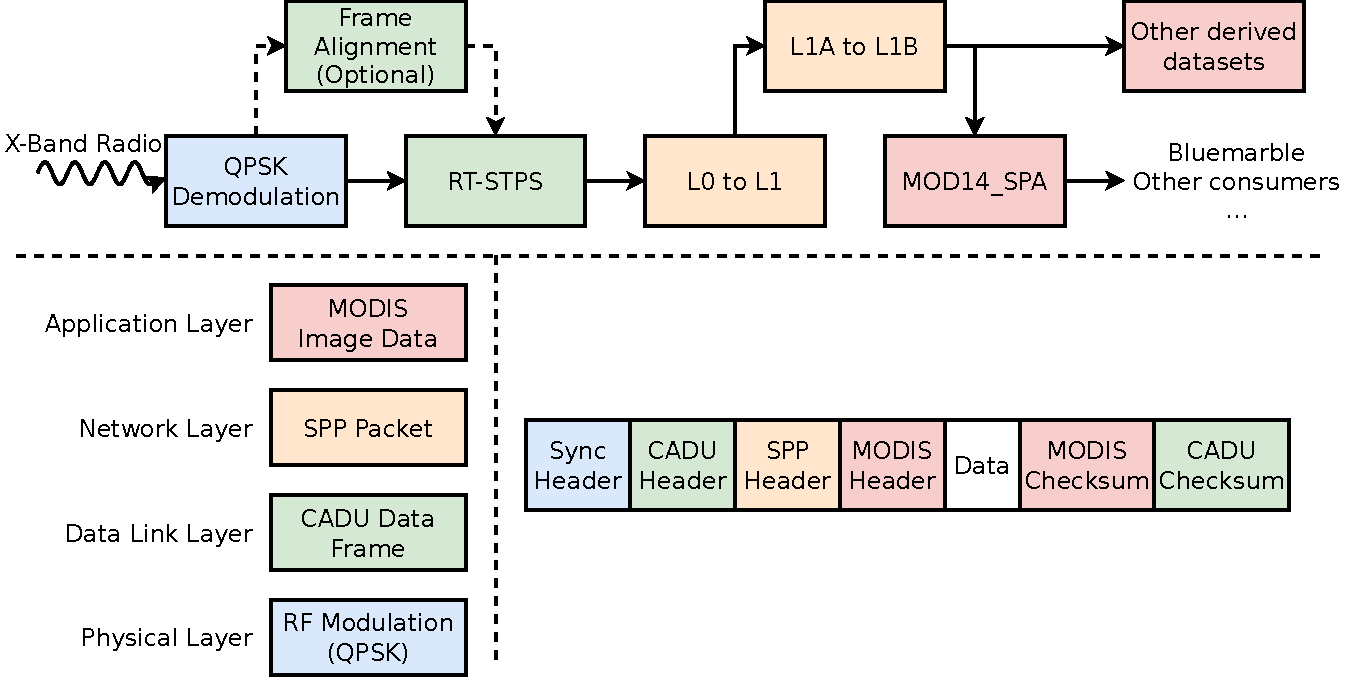
\includegraphics[width=\linewidth]{diagrams/attack_types.pdf}
    \caption{Illustration of the steps involved in processing MODIS image data and derived datasets, as well as the packet structure and layer within the network stack.}
    \label{fig:attack_types}
\end{figure}

% Describe not specific attacks, but the pipeline itself

% NB: we haven't really explained how the different parts of the protocol relate to parts of the packet, and the available attacks

However, in addition to manipulating the instrument data itself, attackers are also able to change protocol-specific fields within the packet headers.
These fields are parsed and used by the initial stages of the processing pipeline to validate and error correct the downlinked signal, and demultiplex and extract the data into an intermediate structure.
As a result, attackers can potentially exploit these early pipeline stages through crafting packets to trigger vulnerabilities.

As a case study we consider NASA's \textit{International Planetary Observation Processing Package} (IPOPP), a software distribution for decoding and processing EOS data.
The software in IPOPP contains protocol decoding stages alongside the satellite-derived dataset generation algorithms.
In particular, the \textit{MODIS Level-1 Science Processing Algorithm} (MODISL1DB\_SPA) is responsible for decoding SPP packets with the MODIS secondary header into the \textit{Heirarchical Data Format} (HDF)~\cite{modisL1DB}.
A summary of the entire pipeline can be found in Figure~\ref{fig:attack_types}.
With a long history going back to the early EOS satellites, the overall system has grown to be incredibly complex, with many interrelating dependencies and execution pathways.
Through overshadowing the signal, an attacker can deliver arbitrary bytes to these processing stages, which were not designed with untrusted input data in mind.

In Section~\ref{sec:evaluation} we consider the effect of a modern adversary against this system.
We demonstrate how the complex execution pathway includes input data being passed between several different processing applications unsafely.
Ultimately, this results in the creation of a payload which gets inserted into the intermediate data structure, and may be triggered by a future reprocessing step.

However, IPOPP is also potentially exploitable due to other well-known vulnerabilities.
Part of the complexity of the system is due to its high number of dependencies, many of which come pre-bundled with the source code.
These dependencies include outdated libraries with documented CVEs (Common Vulnerabilities and Exposures) which haven't been patched.
For example, at the time of writing, MODISL1DB\_SPA comes bundled with HDF5 v1.12.0, which has 11 active CVEs.

% Do I need to explain here exactly what processing stages are involved?

% The code is distributed mixed in with pre-compiled binaries and libraries which are required to make the system work
% Interestingly, Too old for log4shell, for which it is not patched

The extent to which other processing software may be vulnerable to similar attacks is hard to quantify.
However, satellite operators should be aware that similar systems, which may not have been designed to be resilient to untrusted input data, could be exploitable through similar techniques.

\begin{comment}



\textbf{Old stuff below:}

The attacker wants to achieve one of the two objectives
The achieve the first, they must broadcast data that gets decoded correctly.
    This involves understanding any timing,, metadata, etc. is all correct
To achieve the second, they must understand the decoding pipeline
    They are advantaged by weaknesses and lack of standardisation at the data link layer



To attack, yopu neeed to understand the stack
Here's what the stack looks like in general
In our specific case, here's how the protocols look
Move into reencoding

To do so, they must understand the network stack, and have the ability to reencode arbitrary data as a signal that they can overshadow

They need to be able to broadcast at a sufficient strength, such that the receiver decodes it
This is addressed in Section xxx

To the receiver such that it reaches the correct layer in the stack


Split the stack into protocol/data

We discuss a bit about the ecosystem of protocols, with CCSDS SPP forming the common waist, like IP
Data link protocols are less standardized in the space context than OSI model
Fewer security audits, more proprietary software components, making vulnerabilities more likely?

Nod to variety of data link protocols used,

Satellites which roll their own protocols...

% NB: in the case of EOS, we think the only real difference between the downlinks DB and TDRSS is bit rate, from the space shuttle report

% Structure:
%
% Existing software exists (e.g. within IPOPP) to decode satellite signals
% However, no real software exists to encode signals
%
% Prerequisites:
% * Wireless communications packet structure and standards
% * IPOPP pipeline processing stages


The attacker fundamentally needs to overshadow the radio wave with a signal that decodes to the one that they want to inject.
Their aim is the delivery of arbitrary bytes, which will either violate the packet protocol to attempt to exploit a processing step, or cause problems in a satellite-derived dataset.
As a case study, we consider specifically the protocols used in the MODIS downlink of Terra and Aqua, due to the availability of documentation, their representative usage of standard space network layer protocols, and their broad usage in many critical satellite-derived datasets.
We consider how the attacker generates these bytes, the requirements to successfully overshadow the radio wave, and the broader effects of such an attack in Section \ref{sec:evaluation}.

In order to successfully inject bytes, the attacker must provide data that is parsed correctly by the relevant processing steps.
Doing this requires knowledge of the expected packet structure, alongside the processing stages in the pipeline.

\subsection{Terra and Aqua wireless communications specifications} % TODO: different title?

Terra and Aqua communicate on a number of different radio channels and downlink housekeeping, telemetry, and scientific data. \textbf{Are these all the unique ones?}
The satellites themselves can be in one of a number of operational modes, during which they send different information through the available channels. \textbf{TODO: cite SPACE GROUND AQUA document} % TODO: maybe talk about how you can find out more information about this in the appendix?
During nominal operation the satellite is in Direct Broadcast mode, in which the current MODIS sensor data is continuously downlinked.
The data is also buffered for high data rate downlink when the satellite passes over Polar Ground Stations or near its TDRSS relay.

Since the buffer is packed with the same bytes as the Direct Broadcast signal, the format of the data is identical for all modes of broadcast.
We therefore focus on the Direct Broadcast mode without loss of generality.

%To broadcast to the Polar Ground Stations therefore requires a temporary shift out of Direct Broadcast Mode.
%The schedule for direct broadcast can be found for Terra~\cite{terraSchedule} and Aqua~\cite{aquaSchedule} at the HTTP file archive for the Goddard Space Flight Center.

% TODO: describe the structure of each CADU and how the relevant fields e.g. IDs are used
Since each instrument onboard the satellite needs to downlink data simultaneously, the scientific data is sent in a packets to the Formatter/Multiplexer Unit (FMU).
The FMU encapsulates the instrument packets within CCSDS Space Packet Protocol (SPP) packets which contain an Application ID to support demultiplexing per instrument.
The SPP packets are then packed into a custom, unencrypted data link protocol known as the \textit{Channel Access Data Unit}, or CADU.
Finally, the CADUs are modulated onto a radio wave either immediately in the case of Direct Broadcast, or after a short delay for bulk transmission.

\subsection{MODIS downlink decoding pipeline}

On the ground, the signal is received by a tracking satellite antenna and passes through multiple different processing stages to firstly decode the wave into bits, then align the bytes, and finally interpret the data to form satellite-derived datasets.

The data is generally presented to the first software decoding stage as a stream of bits straight from a hardware demodulator component, which therefore presents the first opportunity to exploit a packet decoding stage.

These bits must firstly be byte aligned and divided into CADUs, derandomized through Viterbi decoding depending on the satellite mode, and then error corrected according to the CADU checksum.
These stages are sometimes implemented by dedicated hardware or as a separate piece of software, such as Dartcom's \textit{Polar Orbital Ingester}~\cite{dartcomsystemsltdXBand2021,dartcomPOI}.
However, they can equivalently be handled by NASA's \textit{Real-time Software Telemetry Processing System} (RT-STPS).

In addition to the previous steps, RT-STPS demultiplexes the CADUs and outputs the data they contain, which are in this case SPP packets.
The demultiplexing acts as a basic sanity check, ensuring that each packet has a valid application ID and size.
Through checking at hardcoded bit offsets, RT-STPS also tries to check whether the contents of the CADUs have the correct Application ID.

The resulting data is known as Level 0 data, and contains the demultiplexed CCSDS packets.
The Level 0 data is processed through a pipeline of programs within the IPOPP distribution into subsequently higher levels, eventually resulting in the satellite-derived datasets described in \textbf{TODO: make this table of MODIS data usage}.

\subsubsection{Decoding the packet format}

The Level 0 data consists of SPP packets containing the MODIS instrument packets.
In a single decoding step, the raw sensor readings within the packet are unpacked into a heirarchical data format (HDF), alongside some metadata.

This decoding step is therefore the last chance for an attacker to exploit a processing stage through malformed packet headers.
It is also the point beyond which the satellite-derived datasets are produced, which can be potentially fooled through injecting false or modified data which still conforms to the packet specifications.

%TODO: rephrase this
However, the software is easily exploitable due to some engineering problems


Each program within IPOPP has a standard interface written in XML which describes its available functions and operations.
The XML is parsed by a Java application which runs the available functions through interpreting the available functions using the shell, which generally spawns another program to continue the processing.
Although the interface is common among all IPOPP programs, the programs themselves are very diverse in language and architecture.


The Level 0 data passes through two stages of the \textit{MODIS Level-1 Science Processing Algorithm} (MODISL1DB\_SPA), resulting in heirarchical data format (HDF) files geolocated to a subpixel accuracy.

The first stage, known as \texttt{l0tol1}, processes Level 0 SPP data into Level 1 HDFs, which contains restructured raw sensor samples alongside other metadata.
The second stage, known as \texttt{l1atob}, geolocates the HDFs to a subpixel accuracy using timing information from the data, the satellite's orbital parameters, and an accurate model of the Earth's surface.
The resulting data is considered to be at Level 1B.

Each of these stages relies upon \textit{OceanColor Science Software} (OCSSW)~\cite{ocssw}, written by the OceanColor Data team \textbf{TODO: check}, to perform the actual processing.
In particular, \textbf{TODO: list the tools for each stage} perform the tasks of extracting the data, and correcting corrupted data in the case of failure.
The OCSSW tools are written in C and Fortran, and were originally designed to be run as command line scripts.
They expect a parameter file at a particular relative path \textbf{TODO: check} which itself describes the location of the data to be processed and supplies options for processing it.

In order to automate processing and correcting the data, Python programs were written which construct the command line arguments and parameter files required for the OCSSW tools, and then invoke a shell to execute the tools.
These are designed to be higher-level tools for use in analysing and processing the data files on the command line, which don't require knowledge of the arcane OCSSW formats.

Within IPOPP, \texttt{l0tol1} and \texttt{l1atob} are themselves shell scripts which call these Python programs with certain arguments callable from the XML interface.
\textbf{TODO: fact check that l1atob is actually a shell script and not the Python directly}

\subsubsection{Creating satellite-derived datasets}

% TODO: link to and cite the software manuals and SPA descriptions of each of these
The geolocated Level 1B HDFs proceed into the next processing stage, the \textit{Level 2 MODIS Active Fire Product} (MOD14).
MOD14 identifies active fires from the MODIS data and outputs HDF and txt files considered to be at Level 2. \textbf{TODO: cite manual}

% TODO: describe the structure of MOD14

Through analysing





% TODO: describe granules, and how the raw data gets divided into them?
% TODO: describe the arcane naming convention of the datasets
%   Is this better left for evaluation?

% l0tol1 is distributed twice, there's no version control anywhere
% Reaching out over raw http to servers for data

software within \textit{IPOPP}

% Description of the construction of IPOPP algorithms


%TODO: add details of which things it requires

also demultiplexes the CADUs

After being downconverted and sampled,




\subsection{Encoding arbitrary bytes}

\subsection{Manipulating existing data}




% Wireless spec to go into attack, since it's specific to the MODIS use case
% \subsection{Wireless communications specifications}
% \textit{Discuss the protocols that are used, which will be correlated to later processing stages}

% In each of their downlink modes, \textit{Terra} and \textit{Aqua} communicate using frames modulated onto a carrier wave using quadrature phase shift keying (QPSK).
%In QPSK each symbol (pair of bits) is encoded by shifting the phase of the carrier wave
%In QPSK, symbols represent pairs of bits, and are encoded by shifting the phase of the carrier wave in one of four orientati.

%Information from each of the scientific instruments on the spacecraft is encoded according to the CCSDS packet standard, and are packed into frames known as Channel Access Data Units (CADUs).

%Each CADU is prefixed with a synchronisation header, enabling the receiver software to delimit the frames.
%The rest of the body is "randomized" through XORing with a fixed polynomial to prevent long sequences of the same symbol disrupting transfer.
%The full breakdown of the packet structure can be seen in Fig.~\ref{fig:cadu_diagram}.

%The finalized CADUs are transferred directly to the X-band antenna when in direct broadcast mode, and also to a solid state recorder for playback during the data dumps.


\subsection{Attack description}


Unfortunately the \textit{IPOPP} framework for processing EOS data is open to a variety of attacks through signal injection.
In each case, the attacker leverages different parts of the protocol to redirect the control flow of the program, either causing a denial of service, the leaking of sensitive data, or even arbitrary code execution.

Through the injection of standards-compliant frames, complete with synchronisation headers and checksums, the attacker can convince prior processing stages to decode and demultiplex an arbitrary byte sequence, delivering it as input to \textit{MODISL1DB\_SPA}.

The input to this algorithm is so-called \textit{Level 0} data, which is the body of a data frame with all communications artefacts, including synchronisation headers and checksums, removed.
Through the creation of a custom data frame, the attacker can encapsulate an arbitarary byte sequence which, when overshadowed over the existing signal, will result in the delivery of arbitrary bytes as the input to \textit{MODISL1DB\_SPA}.

We proceed to analyse several classes of attack made possible through this route, and enabled by insecure data handling practices.


\subsection{Exploiting downlink processing systems}

\subsubsection{Unprocessable malformed packets}

The software makes assumptions about the internal structure of the packets, which only hold for benign packets.
With the ability to inject arbitrary data, the attacker can craft packets to exploit oversights in the exception handling code for data parsing, and cause the program to crash.
Since the program processes packets in sets, a single malformed packet is sufficient to prevent the processing of the entire set.

Since the packet data is stored as a dataset for future processing, this attack also lets the attacker poison the dataset to make reprocessing of the entire set significantly harder.


\subsubsection{Latent arbitrary code execution}

In addition to near real-time data processing at the downlinks, past data is often reprocessed to take advantage of new processing alorithms, or to explore new results.
To support these use cases, the processing algorithms within MODISL1DB\_SPA are also available as command line tools, with adjustable configurations.

When run in SPA mode, the configuration used is always the same, which has resulted in a "golden path" through the execution of the program which is relatively secure.
However, by changing the initial configuration, a user could accidentally put the program into a mode which unsafely handles the input data.

Therefore, an attacker can poison the official datasets through the injection of packets, which cause no unsafe behaviour on first processing, but leverage vulnerabilities for arbitrary code execution when reprocessed under a different configuration.
These vulnerabilities have the potential to lie dormant in the official data sources as currently distributed by LAADS DAC, among other Direct Readout stations.

% TODO: go on to demonstrate the attack

\subsubsection{Reading unallocated memory}

Due to the design of the hardware on board the satellite, legitimate communications from the onboard instruments are guaranteed to hold to certain assumptions: for example, the packets are always of the same length, and the internal pointers between the packets are always aligned.

However, in this situation it becomes easy to let implicit assumptions about the structure of the data manifest themselves in the data processing.
Code for handling these exceptional cases is often less rigorously tested, because it generally doesn't occur in benign example cases.

However, by providing shorter packets than expected, with larger pointers than expected, we demonstrate how the attacker can take advantage of certain system components written in C to read off the end of the buffer into unallocated memory.
We demonstrate an execution pathway that would result in the resulting data being stored and uploaded to the public data archives, theoretically allowing the attacker to leak sensitive information from other processes within the memory of the computer.


\subsubsection{Exploiting bundled dependencies}

In order to make software distribution easier, and to create easily deployable systems that mostly "just work" when extracted into a certain location, the IPOPP algorithms generally come with many bundled dependencies in the source archive.
These files are compiled programs and libraries for the handling of input data, that are intended to work on specific architectures.

However, the practice of bundling libraries with software has long been considered bad from a security perspective, especially since the widespread use of package managers to resolve and install dependencies.
Doing so permits a similar ease of installation, but allows each library and program to be traced back to its dependency, independently updated, and uninstalled when no longer required.

Without a system for managing these dependencies, the system becomes incredibly brittle and hard to change; therefore, there are many dependencies currently present and depended upon that haven't been updated in nearly a decade.
Several of these dependencies have patchable security vulnerabilities for arbitrary code execution, that an attacker could take advantage of.

There are also a large number of dependencies that aren't used for any purpose and are just left around for legacy reasons.
Besides potentially being a risk for privilege escalation, the sheer number of redundant dependencies muddies the water and makes it difficult to discern which depencies need updating as a matter of urgency.

% \begin{itemize}
%     \item Strict separation of data handling code from core program control flow
%     \item Secure distribution and patching of dependencies
%     \item Robustness against configuration changes
% \end{itemize}

\end{comment}
